\section{Reinforcement Learning (RL)}\label{sec:rl}
  One of the tried and tested methods of end-to-end learning approaches is a branch under machine learning called \emph{Reinforcement Learning (RL)}. 

  \begin{figure}[h]
    \centering
    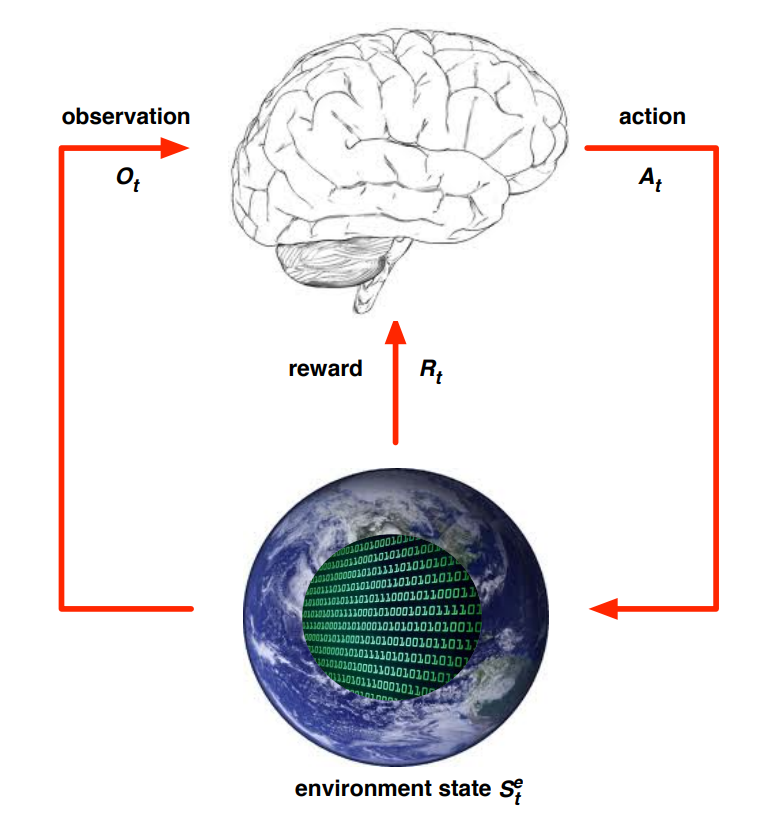
\includegraphics[width=0.6\textwidth]{assets/background/silver-rl.png}
    \caption{Simple RL diagram to reinforce intuition \cite{silver2015}}\label{fig:rl-diag}
  \end{figure}

  RL's main focus is training algorithms, which are called \emph{agents}, in making optimal decisions by interacting with the environment. The key objective is to teach a \emph{policy} to the agent that maximises the overall reward -usually defined by the task and involves a reward or \emph{teacher}. The agent will explore, the possible actions it can take through trial and error, while learning from the feedback given to it by the reward signal and its environment.

  One of the differentiating factors of RL from classical machine learning paradigms is that the feedback is not instantaneous and sequences of decisions influence the subsequent data and signals given to agent \cite{silver2015}.

\subsection{RL in Practice}
  Reinforcement learning, can be used to train a variety of agents that is not limited by physical robots. It can learn to play video-games \cite{comi2018}, automation tasks \cite{} , in natural language processing \cite{paulus2017deepreinforcedmodelabstractive}, applications in healthcare (where RL is categorised as dynamic treatment regimes) for use in chronic diseases or critical care \cite{yu2020reinforcementlearninghealthcaresurvey} and lastly -most importantly for us- learning movement behaviours for robots.

  \subsection{Exploration and Exploitation}
  
  A fundamental challenge in utilising RL is the constant act of balancing \textbf{exploration} and \textbf{exploration}. A trade-off must be made in the created system.
  \begin{enumerate}
    \item \textbf{Exploration:}
    This is when the agent decides to \emph{explore} new actions that might potentially lead to better long-term outcomes. An issue this can cause is that the time it takes to explore all possibilities might not be feasible. But crucial to utilise in in problems with sparse reward models.\todo[color=green]{citations}.
    \item \textbf{Exploitation:}
    When the agent prioritises short-term, immediate rewards by exploiting its current knowledge. For example, taking an agent playing a video game; if a high score was found the agent might be unaware that a higher score can be achieved with a different set of moves. 
  \end{enumerate}

  The trade-offs must be balanced between the two in any RL algorithm or model while considering sampling efficiencies and ease of training \cite{liu2019simpleexplorationsampleefficient}. To relate it back to a robotics example, too much exploration might lead to inefficient training and instability; while too much reliance on exploitation might lead to suboptimal behaviours in the movement of a robot executing a task. 

  % Some common strategies are: $\epsilon$-Greedy, Decay $\epsilon$-Greedy, Upper Confidence Bound (UCB), Thompson Sampling, Intrinsic Motivation (Curiosity-Driven Exploration).
  % \todo[color=green]{citations for these or just remove?}
  
  Along with this widespread use and elemental challenges, comes differing methods of utilising the RL framework. The likes of which can be broadly classified into two types: \textbf{Model-Based} and \textbf{Model-Free}.
  
  \subsection{Model-Based RL}
  Model based approaches involve methods of creating an internal model and representation of the state the agent is interacting with. It usually involves two main steps: learning the dynamics of the model, then planning and learning within it \cite{MAL-086}. These models have underlying principals of the Markov Decision Process (\ref{sec:mdp}).

  Main power of this approach comes from its simulated core. As fewer real interactions can allow it to have a higher sample efficiency \cite{liu2021DRLminireview,wu23robotLearn}, meaning the amount of experience needed (mostly relating to time spent) to learn optimal policies is quite low, and good policies can be quickly learnt.

  On top of that having an underlying model essentially allows the agent to understand its surroundings better, without having to guess or learn them. This means the model can focus on learn the model and generalise better for unseen states \cite{MAL-086}.
  
  However, it also has some drawbacks. Mainly the model introduces a bias into the system, which means inadequate representations or faulty models can create policies that exploit deficiencies in these models \cite{Deisenroth2011PILCO,wang2019benchmarkingmodelbasedreinforcementlearning}, although, some recent works have helped alleviate that bias by characterising the uncertainty of these learnt models \cite{kurutach2018modelensembletrustregionpolicyoptimization,chua2018deepreinforcementlearninghandful,clavera2018modelbasedreinforcementlearningmetapolicy}. Therefore, modelling is a manual, human task which can lead to human-error or insufficient coverage of the action space, leading to suboptimal results.

  One of the most important issues being the learning of the dynamics being coupled with the policy. This makes the agent more prone to performance local-minima, which stem from exploitation and off-learning not being fully investigated under model-based approaches.
  \todo[color=green]{verify this is true and check some sources}

  \subsubsection{Applications in Robotics}
  These methods can be used for motion planning, trajectory optimisation and learning from limited interactions, some common methods are: Monte Carlo Tree Search (MCTS),Probabilistic Inference for Learning Control (PILCO) \cite{Deisenroth2011PILCO}, MuZero: Combines model-based approaches with deep learning.\todo[color=green]{cite here}
  
  \subsection{Model-Free RL}
  This collection of schemes attempt to learn a policy directly by trial and error, without explicitly modelling the environments dynamics. Usually preferred when the environment is too complex or too costly to model.

  There are a few different variants of model-free approaches, all of them similar in the way they omit a model, but have different methods in extracting the optimal policies.
  

  \subsubsection{Value-Based}
  These techniques aim to learn the value of states (or an estimate for the value of states) and actions. So they learn the $v_\pi$ or $q_\pi$ function. which can then be used to extract the optimal policy $\pi_*$ for deciding the actions.

  Such systems are mainly used for simple navigation tasks, basic motor control and arm reaching scenarios. Some example methods are: Q-Learning [Off-Policy], Deep Q-Networks (DQN) [Off-Policy], SARSA [On-Policy]. \todo[color=green]{citations}

  \subsubsection{Policy-Based}
  This on the other hand learn a policy directly. Bypassing the need to learn the values of states or actions completely. This can be helpful if the state space and/or the action space are quite large. For example, if the action space was infinite, then value-based approaches would not be feasible as all actions must be tried to find the best, which makes directly learning the policy is the only possible approach.

  These systems are for more complex control tasks, such as dexterous limb manipulation, robot hand grasping. Some examples are: REINFORCE [On-Policy], Proximal Policy Optimisation (PRO) [On-Policy], Trust Region Policy Optimisation (TRPO) [On-Policy]. \todo[color=green]{citations}

  \subsubsection{Actor-Teacher} 
  The main idea in this approach is the agent improves its policy from direct feedback from a \emph{teacher}, this teacher can be an external system that provides rewards or a complete manual system where the teacher is an ``expert human'' providing demonstrations (which goes into Imitation Learning, see \ref{sec:il}). Some common approaches are
  \begin{itemize}
    \item \textbf{Direct Action Supervision}: where the teacher suggest actions directly to the agent.
    \item \textbf{Criticising Actions}: where the actions are suggested by the teacher.\todo{not sure if this makes sense}
    \item \textbf{Shaped Rewards}: the teacher modifies the reward signal dynamically to encourage desirable behaviours.
    \item \textbf{Curriculum Learning}: the teacher controls the difficulty of tasks over time to ease the learning of the agent.
  \end{itemize}
  
  \subsubsection{Hybrid Approaches}
  Mixing the two together is also a viability, where the characteristics from each can be combined benefit from different guarantees each provides \cite{qu2020combiningmodelbasedmodelfreemethods}
  On top of the model dependence, the RL approach can be of two flavours:

  \subsection{On-Policy}
  This approach means that the agent updates its policy from data generated by the current policy. So an agent can only learn from the actions it purposefully took under its latest policy. Which can restrict improvements, but means that no outdated or stale data can influence the present time actions or learning.
  This leads to more stable learning in stochastic environments \todo[color=green]{citation?} while ensuring policy consistency.

  However, it also means that the agent becomes sample inefficient, as fresh iterations are needed to learn and sharpen the current policy. On top of that, the learning rate slows down because the agent can't use older experience (only the latest policy), slowing training \cite{andrychowicz2020onpolicyRL}.

  \subsection{Off-Policy}
  In this case, the agent can utilise past experiences, regardless of the policy generated by the training. This recycling of information previously known makes the learning more efficient \cite{uehara2022reviewoffpolicyevaluationreinforcement}, as sample efficiency is increased.
  Having past experiences also means that the agent will need fewer exploration steps and less iterations because of these priors. Making this system efficient in deterministic environments. \todo[color=green]{not quite sure why, add here}
  
  This however, brings instability in stochastic environments, and the the policy diverging due to incorporating outdated and possibly uninformative (at least at the present) data. Therefore, some sort of importance of older steps should be kept track of, and maybe even decayed like the discount factor from MDPs (\ref{sec:mdp}). \cite{maroti2019rbed} \todo{check this evidence not sure, and link to earlier}
  \\\\
  Both of these approaches can be combined with either \textbf{Model-Based} or \textbf{Model-Free} approaches. Because at the end of the day, making a good model is about picking the correct trade-offs that is relevant to the scenario of the problem we are attempting to solve.
